\documentclass[aspectratio=169]{beamer}\usepackage[]{graphicx}\usepackage[]{xcolor}
% maxwidth is the original width if it is less than linewidth
% otherwise use linewidth (to make sure the graphics do not exceed the margin)
\makeatletter
\def\maxwidth{ %
  \ifdim\Gin@nat@width>\linewidth
    \linewidth
  \else
    \Gin@nat@width
  \fi
}
\makeatother

\definecolor{fgcolor}{rgb}{0.345, 0.345, 0.345}
\newcommand{\hlnum}[1]{\textcolor[rgb]{0.686,0.059,0.569}{#1}}%
\newcommand{\hlsng}[1]{\textcolor[rgb]{0.192,0.494,0.8}{#1}}%
\newcommand{\hlcom}[1]{\textcolor[rgb]{0.678,0.584,0.686}{\textit{#1}}}%
\newcommand{\hlopt}[1]{\textcolor[rgb]{0,0,0}{#1}}%
\newcommand{\hldef}[1]{\textcolor[rgb]{0.345,0.345,0.345}{#1}}%
\newcommand{\hlkwa}[1]{\textcolor[rgb]{0.161,0.373,0.58}{\textbf{#1}}}%
\newcommand{\hlkwb}[1]{\textcolor[rgb]{0.69,0.353,0.396}{#1}}%
\newcommand{\hlkwc}[1]{\textcolor[rgb]{0.333,0.667,0.333}{#1}}%
\newcommand{\hlkwd}[1]{\textcolor[rgb]{0.737,0.353,0.396}{\textbf{#1}}}%
\let\hlipl\hlkwb

\usepackage{framed}
\makeatletter
\newenvironment{kframe}{%
 \def\at@end@of@kframe{}%
 \ifinner\ifhmode%
  \def\at@end@of@kframe{\end{minipage}}%
  \begin{minipage}{\columnwidth}%
 \fi\fi%
 \def\FrameCommand##1{\hskip\@totalleftmargin \hskip-\fboxsep
 \colorbox{shadecolor}{##1}\hskip-\fboxsep
     % There is no \\@totalrightmargin, so:
     \hskip-\linewidth \hskip-\@totalleftmargin \hskip\columnwidth}%
 \MakeFramed {\advance\hsize-\width
   \@totalleftmargin\z@ \linewidth\hsize
   \@setminipage}}%
 {\par\unskip\endMakeFramed%
 \at@end@of@kframe}
\makeatother

\definecolor{shadecolor}{rgb}{.97, .97, .97}
\definecolor{messagecolor}{rgb}{0, 0, 0}
\definecolor{warningcolor}{rgb}{1, 0, 1}
\definecolor{errorcolor}{rgb}{1, 0, 0}
\newenvironment{knitrout}{}{} % an empty environment to be redefined in TeX

\usepackage{alltt}



\usetheme{default}
% Slide setup, colour independent

\usepackage{amsmath,amssymb,amsthm}
\usepackage[utf8]{inputenc}
\usepackage{colortbl}
\usepackage{bm}
\usepackage{xcolor}
\usepackage{dsfont}
\usepackage{setspace}
% To use \ding{234} and the like
\usepackage{pifont}
% To cross reference between slide files
\usepackage{zref-xr,zref-user}
% Use something like
% \zexternaldocument{fileI}
% in the tex files. And cite using \zref instead of \ref
\usepackage{booktabs}
\usepackage{marvosym}
\usepackage{cancel}
%\usepackage{transparent}
% Make doi clickable in the bibliography?
\usepackage{doi}

\usepackage[T1]{fontenc}

\usepackage{longtable}

% For heavier titles
\usepackage{helvet} % Enables Helvetica font family


% Fields and the like
\def\IC{\mathbb{C}}
\def\IE{\mathbb{E}}
\def\IF{\mathbb{F}}
\def\II{\mathbb{I}}
\def\IJ{\mathbb{J}}
\def\IK{\mathbb{K}}
\def\IM{\mathbb{M}}
\def\IN{\mathbb{N}}
\def\IP{\mathbb{P}}
\def\IR{\mathbb{R}}
\newcommand{\IRplus}{\mathbb{R}_{\ge 0}}
\def\IZ{\mathbb{Z}}
\def\11{\mathds{1}}


% Bold lowercase
\def\ba{\bm{a}}
\def\bb{\bm{b}}
\def\bc{\bm{c}}
\def\bd{\bm{d}}
\def\be{\bm{e}}
\def\bf{\bm{f}}
\def\bg{\bm{g}}
\def\bh{\bm{h}}
\def\bi{\bm{i}}
\def\bj{\bm{j}}
\def\bk{\bm{k}}
\def\bn{\bm{n}}
\def\bp{\bm{p}}
\def\br{\bm{r}}
\def\bs{\bm{s}}
\def\bu{\bm{u}}
\def\bv{\bm{v}}
\def\bw{\bm{w}}
\def\bx{\bm{x}}
\def\by{\bm{y}}
\def\bz{\bm{z}}
\newcommand{\vect}[1]{\bm{#1}}

% Bold capitals
\def\bB{\bm{B}}
\def\bD{\bm{D}}
\def\bE{\bm{E}}
\def\bF{\bm{F}}
\def\bG{\bm{G}}
\def\bI{\bm{I}}
\def\bL{\bm{L}}
\def\bN{\bm{N}}
\def\bP{\bm{P}}
\def\bR{\bm{R}}
\def\bS{\bm{S}}
\def\bT{\bm{T}}
\def\bX{\bm{X}}

% Bold numbers
\def\b0{\bm{0}}

% Bold greek
\bmdefine{\bmu}{\bm{\mu}}
\def\bphi{\bm{\phi}}
\def\bvarphi{\bm{\varphi}}
\def\bPi{\bm{\Pi}}
\def\bGamma{\bm{\Gamma}}

% Bold red sentence
\def\boldred#1{{\color{red}\textbf{#1}}}
\def\defword#1{{\color{orange}\textbf{#1}}}

% Caligraphic letters
\def\A{\mathcal{A}}
\def\B{\mathcal{B}}
\def\C{\mathcal{C}}
\def\D{\mathcal{D}}
\def\E{\mathcal{E}}
\def\F{\mathcal{F}}
\def\G{\mathcal{G}}
\def\H{\mathcal{H}}
\def\I{\mathcal{I}}
\def\L{\mathcal{L}}
\def\M{\mathcal{M}}
\def\N{\mathcal{N}}
\def\P{\mathcal{P}}
\def\R{\mathcal{R}}
\def\S{\mathcal{S}}
\def\T{\mathcal{T}}
\def\U{\mathcal{U}}
\def\V{\mathcal{V}}

% Adding space for prime (') where needed
\def\pprime{\,'}
% Adding space for star (\star) where needed
\def\pstar{{\,\star}}

% tt font for code
\def\code#1{{\tt #1}}

% i.e., e.g.
\def\eg{\emph{e.g.}}
\def\ie{\emph{i.e.}}


% Operators and special symbols
\def\nbOne{{\mathchoice {\rm 1\mskip-4mu l} {\rm 1\mskip-4mu l}
{\rm 1\mskip-4.5mu l} {\rm 1\mskip-5mu l}}}
\def\cov{\ensuremath{\mathsf{cov}}}
\def\Var{\ensuremath{\mathsf{Var}\ }}
\def\Im{\textrm{Im}\;}
\def\Re{\textrm{Re}\;}
\def\det{\ensuremath{\mathsf{det}}}
\def\diag{\ensuremath{\mathsf{diag}}}
\def\nullspace{\ensuremath{\mathsf{null}}}
\def\nullity{\ensuremath{\mathsf{nullity}}}
\def\rank{\ensuremath{\mathsf{rank}}}
\def\range{\ensuremath{\mathsf{range}}}
\def\sgn{\ensuremath{\mathsf{sgn}}}
\def\Span{\ensuremath{\mathsf{span}}}
\def\tr{\ensuremath{\mathsf{tr}}}
\def\imply{$\Rightarrow$}
\def\restrictTo#1#2{\left.#1\right|_{#2}}
\newcommand{\parallelsum}{\mathbin{\!/\mkern-5mu/\!}}
\def\dsum{\mathop{\displaystyle \sum }}%
\def\dind#1#2{_{\substack{#1\\ #2}}}

\newcommand{\Qmatrix}[1]{%
  \begin{pmatrix}#1\end{pmatrix}%
}

\DeclareMathOperator{\GL}{GL}
\DeclareMathOperator{\Rel}{Re}
\def\Nt#1{\left|\!\left|\!\left|#1\right|\!\right|\!\right|}
\newcommand{\tripbar}{|\! |\! |}



% The beamer bullet (in base colour)
\def\bbullet{\leavevmode\usebeamertemplate{itemize item}\ }

% Theorems and the like
\newtheorem{proposition}[theorem]{Proposition}
\newtheorem{property}[theorem]{Property}
\newtheorem{importantproperty}[theorem]{Property}
\newtheorem{importanttheorem}[theorem]{Theorem}
%\newtheorem{lemma}[theorem]{Lemma}
%\newtheorem{corollary}[theorem]{Corollary}
\newtheorem{remark}[theorem]{Remark}
\setbeamertemplate{theorems}[numbered]
%\setbeamertemplate{theorems}[ams style]

%
%\usecolortheme{orchid}
%\usecolortheme{orchid}

\def\red{\color[rgb]{1,0,0}}
\def\blue{\color[rgb]{0,0,1}}
\def\green{\color[rgb]{0,1,0}}

% Fix skipping lines after items in the bibliography
\setbeamertemplate{bibliography entry title}{}
\setbeamertemplate{bibliography entry location}{}
\setbeamertemplate{bibliography entry note}{}

% Get rid of navigation stuff
\setbeamertemplate{navigation symbols}{}

% Set footline/header line
\setbeamertemplate{footline}
{%
\quad p. \insertpagenumber \quad--\quad \insertsection\vskip2pt
}
% \setbeamertemplate{headline}
% {%
% \quad\insertsection\hfill p. \insertpagenumber\quad\mbox{}\vskip2pt
% }


\makeatletter
\newlength\beamerleftmargin
\setlength\beamerleftmargin{\Gm@lmargin}
\makeatother

% Colours for special pages
\def\extraContent{yellow!20}


%%%%%%%%%%%%%%%%%
\usepackage{tikz}
\usetikzlibrary{shapes,arrows}
\usetikzlibrary{positioning}
\usetikzlibrary{shapes.symbols,shapes.callouts,patterns}
\usetikzlibrary{calc,fit}
\usetikzlibrary{backgrounds}
\usetikzlibrary{decorations.pathmorphing,fit,petri}
\usetikzlibrary{automata}
\usetikzlibrary{fadings}
\usetikzlibrary{patterns,hobby}
\usetikzlibrary{backgrounds,fit,petri}
\usetikzlibrary{tikzmark}

\usepackage{pgfplots}
\pgfplotsset{compat=1.6}
\pgfplotsset{ticks=none}

\usetikzlibrary{decorations.markings}
\usetikzlibrary{arrows.meta}
\tikzset{>=stealth}

% For tikz
\tikzstyle{cloud} = [draw, ellipse,fill=red!20, node distance=0.87cm,
minimum height=2em]
\tikzstyle{line} = [draw, -latex']


%%% For max frame images
\newenvironment{changemargin}[2]{%
\begin{list}{}{%
\setlength{\topsep}{0pt}%
\setlength{\leftmargin}{#1}%
\setlength{\rightmargin}{#2}%
\setlength{\listparindent}{\parindent}%
\setlength{\itemindent}{\parindent}%
\setlength{\parsep}{\parskip}%
}%
\item[]}{\end{list}}


% Make one image take up the entire slide content area in beamer,.:
% centered/centred full-screen image, with title:
% This uses the whole screen except for the 1cm border around it
% all. 128x96mm
\newcommand{\titledFrameImage}[2]{
\begin{frame}{#1}
%\begin{changemargin}{-1cm}{-1cm}
\begin{center}
\includegraphics[width=108mm,height=\textheight,keepaspectratio]{#2}
\end{center}
%\end{changemargin}
\end{frame}
}

% Make one image take up the entire slide content area in beamer.:
% centered/centred full-screen image, no title:
% This uses the whole screen except for the 1cm border around it
% all. 128x96mm
\newcommand{\plainFrameImage}[1]{
\begin{frame}[plain]
%\begin{changemargin}{-1cm}{-1cm}
\begin{center}
\includegraphics[width=108mm,height=76mm,keepaspectratio]{#1}
\end{center}
%\end{changemargin}
\end{frame}
}

% Make one image take up the entire slide area, including borders, in beamer.:
% centered/centred full-screen image, no title:
% This uses the entire whole screen
\newcommand{\maxFrameImage}[1]{
\begin{frame}[plain]
\begin{changemargin}{-1cm}{-1cm}
\begin{center}
\includegraphics[width=\paperwidth,height=\paperheight,keepaspectratio]
{#1}
\end{center}
\end{changemargin}
\end{frame}
}

% This uses the entire whole screen (to include in frame)
\newcommand{\maxFrameImageNoFrame}[1]{
\begin{changemargin}{-1cm}{-1cm}
\begin{center}
\includegraphics[width=\paperwidth,height=0.99\paperheight,keepaspectratio]
{#1}
\end{center}
\end{changemargin}
}

% Make one image take up the entire slide area, including borders, in beamer.:
% centered/centred full-screen image, no title:
% This uses the entire whole screen
\newcommand{\maxFrameImageColor}[2]{
\begin{frame}[plain]
\setbeamercolor{normal text}{bg=#2!20}
\begin{changemargin}{-1cm}{-1cm}
\begin{center}
\includegraphics[width=\paperwidth,height=\paperheight,keepaspectratio]
{#1}
\end{center}
\end{changemargin}
\end{frame}
}


\usepackage{tikz}
\usetikzlibrary{patterns,hobby}
\usepackage{pgfplots}
\pgfplotsset{compat=1.6}
\pgfplotsset{ticks=none}

\usetikzlibrary{backgrounds}
\usetikzlibrary{decorations.markings}
\usetikzlibrary{arrows.meta}
\tikzset{>=stealth}

\tikzset{
  clockwise arrows/.style={
    postaction={
      decorate,
      decoration={
        markings,
        mark=between positions 0.1 and 0.9 step 40pt with {\arrow{>}},
   }}}}


% Beginning of a section
\newcommand{\newSectionSlide}[1]{
\begin{frame}[noframenumbering,plain]
  \begin{tikzpicture}[remember picture,overlay]
    \node[above right,inner sep=0pt,opacity=0.2] at (current page.south west)
    {
        \includegraphics[height=\paperheight,width=\paperwidth]{#1}
    };
  \end{tikzpicture}
  \setbeamercolor{section in toc}{fg=section_page_list_colour}
  \setbeamerfont{section in toc}{size=\Large,series=\bfseries}
  \setbeamertemplate{section in toc shaded}[default][60]
  \tableofcontents[
    currentsection,
    sectionstyle=show/shaded,
    subsectionstyle=show/hide/hide,
    subsubsectionstyle=hide/hide/hide]
\end{frame}
\addtocounter{page}{-1}
}

% Beginning of a section in which we also show subsections
\newcommand{\newSectionWithSubsSlide}[1]{
	\begin{frame}[noframenumbering,plain]
		\begin{tikzpicture}[remember picture,overlay]
			\node[above right,inner sep=0pt,opacity=0.2] at (current page.south west)
			{
				\includegraphics[height=\paperheight,width=\paperwidth]{#1}
			};
		\end{tikzpicture}
		\setbeamercolor{section in toc}{fg=section_page_list_colour}
		\setbeamerfont{section in toc}{size=\Large,series=\bfseries}
		\setbeamertemplate{section in toc shaded}[default][60]
		\tableofcontents[
		currentsection,
		sectionstyle=show/hide,
		subsectionstyle=show/show/hide,
		subsubsectionstyle=hide/hide/hide]
	\end{frame}
	\addtocounter{page}{-1}
}

% Beginning of a subsection
\newcommand{\newSubSectionSlide}[1]{
\begin{frame}[noframenumbering,plain]
  \begin{tikzpicture}[remember picture,overlay]
    \node[above right,inner sep=0pt,opacity=0.2] at (current page.south west)
    {
        \includegraphics[height=\paperheight,width=\paperwidth]{#1}
    };
  \end{tikzpicture}
  \setbeamercolor{section in toc}{fg=subsection_page_list_colour}
  \setbeamerfont{section in toc}{size=\Large,series=\bfseries}
  \setbeamertemplate{section in toc shaded}[default][60]
  \setbeamerfont{subsection in toc}{series=\bfseries}
  \setbeamertemplate{subsection in toc shaded}[default][50]
  \tableofcontents[
    currentsection,
    sectionstyle=show/hide,
    subsectionstyle=show/shaded/hide,
    subsubsectionstyle=hide/hide/hide]
\end{frame}
\addtocounter{page}{-1}
}


% Beginning of a subsubsection
\newcommand{\newSubSubSectionSlide}[1]{
\begin{frame}[noframenumbering,plain]
  \begin{tikzpicture}[remember picture,overlay]
    \node[above right,inner sep=0pt,opacity=0.2] at (current page.south west)
    {
        \includegraphics[height=\paperheight,width=\paperwidth]{#1}
    };
  \end{tikzpicture}
  \setbeamercolor{section in toc}{fg=subsub_header_section}
  \setbeamerfont{section in toc}{size=\Large,series=\bfseries}
  \setbeamertemplate{section in toc shaded}[default][60]
  \setbeamerfont{subsection in toc}{series=\bfseries}
  \setbeamertemplate{subsection in toc shaded}[default][50]
  \setbeamertemplate{subsubsection in toc shaded}[default][50]
  \tableofcontents[
    currentsection,
    sectionstyle=show/hide,
    subsectionstyle=show/hide/hide,
    subsubsectionstyle=show/shaded/hide]
\end{frame}
\addtocounter{page}{-1}
}


   %%%%%%%%%%%
% To have links to parts in the outline
\makeatletter
\AtBeginPart{%
  \addtocontents{toc}{\protect\beamer@partintoc{\the\c@part}{\beamer@partnameshort}{\the\c@page}}%
}
%% number, shortname, page.
\providecommand\beamer@partintoc[3]{%
  \ifnum\c@tocdepth=-1\relax
    % requesting onlyparts.
    \makebox[6em]{Part #1:} \textcolor{green!30!blue}{\hyperlink{#2}{#2}}
    \par
  \fi
}
\define@key{beamertoc}{onlyparts}[]{%
  \c@tocdepth=-1\relax
}
\makeatother%

\newcommand{\nameofthepart}{}
\newcommand{\nupart}[1]%
    {   \part{#1}%
        \renewcommand{\nameofthepart}{#1}%
        {
          \setbeamercolor{background canvas}{bg=orange!50}
          \begin{frame}{#1}%\partpage 
          \hypertarget{\nameofthepart}{}\tableofcontents%
          \end{frame}
        }
    }

% This command creates a title page using TikZ only
\newcommand{\tikztitlepage}[1]{%
\begin{frame}[plain,noframenumbering]
  \begin{tikzpicture}[remember picture,overlay]
    % Background image
    \node[above right,inner sep=0pt,opacity=0.1] 
      at (current page.south west) 
      {\includegraphics[width=\paperwidth,height=\paperheight]{#1}};

    % University logo
    \node[anchor=north east, inner sep=5pt, opacity=0.9] 
      at (current page.north east)
      {
\includegraphics[width=0.2\textwidth]{FIGS-slides-admin/UM-logo-horizontal-CMYK.png}};
    
    % Title
    \node[anchor=center, align=center, 
          font=\fontsize{13}{15}\bfseries\color{UMbrown}, 
          text width=0.9\textwidth] 
          at ([yshift=2cm]current page.center)
          {\inserttitle};

      % Authors
      \node[anchor=center, align=center,
        font=\fontsize{10}{12}\bfseries\color{UMbrown},
        text width=0.7\textwidth]
        at ([yshift=0.8cm]current page.center)
        {\insertauthor};

      % Affiliation
      \node[anchor=north, align=center,
        font=\fontsize{9}{11}\color{UMbrown},
        text width=0.7\textwidth]
        at ([yshift=-0.2cm]current page.center)
        {\insertaffiliation};      
    % Date
    \node[anchor=north, align=center, 
          font=\fontsize{12}{16}\bfseries\color{UMbrown},
          text width=0.7\textwidth] 
          at ([yshift=0.2cm]current page.center)
          {\insertdate};

    % Land acknowledgement
    \node[anchor=south, align=justify, 
          font=\footnotesize, text=black, 
          text width=1.1\textwidth] 
          at ([yshift=0.5cm]current page.south)
          {The University of Manitoba campuses are located on original lands of Anishinaabeg, Ininew, Anisininew, Dakota and Dene peoples, and on the National Homeland of the Red River Métis.\\
          We respect the Treaties that were made on these territories, we acknowledge the harms and mistakes of the past, and we dedicate ourselves to move forward in partnership with Indigenous communities in a spirit of Reconciliation and collaboration.};
  \end{tikzpicture}
  \addtocounter{page}{-1}
\end{frame}
}
% The title page with figure
% \newcommand{\titlepagewithfigure}[1]{%
%   \begin{frame}[noframenumbering,plain]
%     \begin{tikzpicture}[remember picture,overlay]
%       \node[above right,inner sep=0pt,opacity=0.1] at (current page.south west)
%       {
%           \includegraphics[height=\paperheight,width=\paperwidth]{#1}
%       };
%       \node[anchor=north east,
%       inner sep=5pt,
%       opacity=0.9] at (current page.north east)
%       {
%           
\includegraphics[width=0.2\textwidth]{FIGS-slides-admin/UM-logo-horizontal-CMYK.png}
%       };
%       \node[anchor=south, 
%       align=justify, 
%       text=black, 
%       text width=1.1\textwidth,
%       font=\footnotesize]  (land_acknowledgement)
%       at (current page.south) 
%       {The University of Manitoba campuses are located on original lands of Anishinaabeg, Ininew, Anisininew, Dakota and Dene peoples, and on the National Homeland of the Red River Métis.
%       We respect the Treaties that were made on these territories, we acknowledge the harms and mistakes of the past, and we dedicate ourselves to move forward in partnership with Indigenous communities in a spirit of Reconciliation and collaboration.};  
%       % \node[align=center, anchor=south,
%       % above=0.5cm of land_acknowledgement,
%       % text=black,
%       % font=\bfseries] {\insertdate};
%   \end{tikzpicture}
%   \setbeamercolor{title}{fg=title_page_title_colour}
%   \setbeamerfont{title}{size=\Large,series=\bfseries}
%   \setbeamercolor{author}{fg=title_page_author_colour}
%   \setbeamerfont{author}{size=\large,series=\bfseries}
%   \setbeamercolor{institute}{fg=title_page_institute_colour}
%   \setbeamerfont{institute}{size=\large,series=\bfseries}
%   \setbeamercolor{date}{fg=title_page_date_colour}
%   \setbeamerfont{date}{series=\bfseries}
% 	\titlepage
% \end{frame}
% \addtocounter{page}{-1}
% }

\newcommand{\titlepagewithfigure}[1]{%
  \begin{frame}[noframenumbering,plain]
    \begin{tikzpicture}[remember picture,overlay]
      \node[above right,inner sep=0pt,opacity=0.1] at (current page.south west)
      {
          \includegraphics[height=\paperheight,width=\paperwidth]{#1}
      };
      \node[anchor=north east,
      inner sep=5pt,
      opacity=0.9] at (current page.north east)
      {
          
\includegraphics[width=0.2\textwidth]{FIGS-slides-admin/UM-logo-horizontal-CMYK.png}
      };
      \node[anchor=south, 
      align=justify, 
      text=black, 
      text width=1.1\textwidth,
      font=\footnotesize]  (land_acknowledgement)
      at (current page.south) 
      {The University of Manitoba campuses are located on original lands of Anishinaabeg, Ininew, Anisininew, Dakota and Dene peoples, and on the National Homeland of the Red River Métis.
      We respect the Treaties that were made on these territories, we acknowledge the harms and mistakes of the past, and we dedicate ourselves to move forward in partnership with Indigenous communities in a spirit of Reconciliation and collaboration.};  
      % \node[align=center, anchor=south,
      % above=0.5cm of land_acknowledgement,
      % text=black,
      % font=\bfseries] {\insertdate};
  \end{tikzpicture}
  \setbeamercolor{title}{fg=title_page_title_colour}
  \setbeamerfont{title}{size=\Large,series=\bfseries,family=\usefont{T1}{phv}{b}{n}}
  \setbeamercolor{author}{fg=title_page_author_colour}
  \setbeamerfont{author}{size=\large,series=\bfseries,family=\usefont{T1}{phv}{b}{n}}
  \setbeamercolor{institute}{fg=title_page_institute_colour}
  \setbeamerfont{institute}{size=\large,series=\bfseries,family=\usefont{T1}{phv}{b}{n}}
  \setbeamercolor{date}{fg=title_page_date_colour}
  \setbeamerfont{date}{series=\bfseries,family=\usefont{T1}{phv}{b}{n}}
	\titlepage
\end{frame}
\addtocounter{page}{-1}
}
% The outline page, with figure
% \newcommand{\outlinepage}[1]{%
% \begin{frame}[noframenumbering,plain]
%   \begin{tikzpicture}[remember picture,overlay]
%     \node[above right,inner sep=0pt,opacity=0.2] at (current page.south west)
%     {
%         \includegraphics[height=\paperheight,width=\paperwidth]{#1}
%     };
%   \end{tikzpicture}
%   \setbeamercolor{section in toc}{fg=outline_page_list_colour}
%   \setbeamerfont{section in toc}{size=\Large,series=\bfseries,family=\sffamily}
%   \frametitle{\textcolor{outline_page_title_colour}{\LARGE\bfseries Outline}}
%   \tableofcontents[hideallsubsections]
% \end{frame}
% \addtocounter{page}{-1}
% }
% The outline page, with figure
\newcommand{\outlinepage}[1]{%
\begin{frame}[noframenumbering,plain]
  \begin{tikzpicture}[remember picture,overlay]
    \node[above right,inner sep=0pt,opacity=0.2] at (current page.south west)
    {
        \includegraphics[height=\paperheight,width=\paperwidth]{#1}
    };
  \end{tikzpicture}
  \setbeamercolor{section in toc}{fg=outline_page_list_colour}
  % Use Helvetica Bold only for the outline slide TOC
  \setbeamerfont{section in toc}{size=\Large,family=\usefont{T1}{phv}{b}{n}}
  % Use Helvetica Bold for the outline title
  \frametitle{\textcolor{outline_page_title_colour}{\usefont{T1}{phv}{b}{n}\LARGE Outline}}
  \tableofcontents[hideallsubsections]
\end{frame}
\addtocounter{page}{-1}
}


%\let\oldsection\section
%\renewcommand{\section}[2]{\oldsection[#1]\newSectionSlide[#2]}





\usecolortheme{orchid}
%% Listings
\usepackage{listings}
\definecolor{mygreen}{rgb}{0,0.6,0}
\definecolor{mygray}{rgb}{0.5,0.5,0.5}
\definecolor{mymauve}{rgb}{0.58,0,0.82}
\definecolor{mygold}{rgb}{1,0.843,0}
\definecolor{myblue}{rgb}{0.537,0.812,0.941}

\definecolor{mygold2}{RGB}{120,105,22}
\definecolor{mygrey2}{RGB}{50,50,50}

\definecolor{lgreen}{rgb}{0.6,0.9,.6}
\definecolor{lred}{rgb}{1,0.5,.5}

\lstloadlanguages{R}
\lstset{ %
  language=R,
  backgroundcolor=\color{black!05},   % choose the background color
  basicstyle=\footnotesize\ttfamily,        % size of fonts used for the code
  breaklines=true,                 % automatic line breaking only at whitespace
  captionpos=b,                    % sets the caption-position to bottom
  commentstyle=\color{mygreen},    % comment style
  escapeinside={\%*}{*)},          % if you want to add LaTeX within your code
  keywordstyle=\color{red},       % keyword style
  stringstyle=\color{mygold},     % string literal style
  keepspaces=true,
  columns=fullflexible,
  tabsize=4,
}
% Could also do (in lstset)
% basicstyle==\fontfamily{pcr}\footnotesize
\lstdefinelanguage{Renhanced}%
  {keywords={abbreviate,abline,abs,acos,acosh,action,add1,add,%
      aggregate,alias,Alias,alist,all,anova,any,aov,aperm,append,apply,%
      approx,approxfun,apropos,Arg,args,array,arrows,as,asin,asinh,%
      atan,atan2,atanh,attach,attr,attributes,autoload,autoloader,ave,%
      axis,backsolve,barplot,basename,besselI,besselJ,besselK,besselY,%
      beta,binomial,body,box,boxplot,break,browser,bug,builtins,bxp,by,%
      c,C,call,Call,case,cat,category,cbind,ceiling,character,char,%
      charmatch,check,chol,chol2inv,choose,chull,class,close,cm,codes,%
      coef,coefficients,co,col,colnames,colors,colours,commandArgs,%
      comment,complete,complex,conflicts,Conj,contents,contour,%
      contrasts,contr,control,helmert,contrib,convolve,cooks,coords,%
      distance,coplot,cor,cos,cosh,count,fields,cov,covratio,wt,CRAN,%
      create,crossprod,cummax,cummin,cumprod,cumsum,curve,cut,cycle,D,%
      data,dataentry,date,dbeta,dbinom,dcauchy,dchisq,de,debug,%
      debugger,Defunct,default,delay,delete,deltat,demo,de,density,%
      deparse,dependencies,Deprecated,deriv,description,detach,%
      dev2bitmap,dev,cur,deviance,off,prev,,dexp,df,dfbetas,dffits,%
      dgamma,dgeom,dget,dhyper,diag,diff,digamma,dim,dimnames,dir,%
      dirname,dlnorm,dlogis,dnbinom,dnchisq,dnorm,do,dotplot,double,%
      download,dpois,dput,drop,drop1,dsignrank,dt,dummy,dump,dunif,%
      duplicated,dweibull,dwilcox,dyn,edit,eff,effects,eigen,else,%
      emacs,end,environment,env,erase,eval,equal,evalq,example,exists,%
      exit,exp,expand,expression,External,extract,extractAIC,factor,%
      fail,family,fft,file,filled,find,fitted,fivenum,fix,floor,for,%
      For,formals,format,formatC,formula,Fortran,forwardsolve,frame,%
      frequency,ftable,ftable2table,function,gamma,Gamma,gammaCody,%
      gaussian,gc,gcinfo,gctorture,get,getenv,geterrmessage,getOption,%
      getwd,gl,glm,globalenv,gnome,GNOME,graphics,gray,grep,grey,grid,%
      gsub,hasTsp,hat,heat,help,hist,home,hsv,httpclient,I,identify,if,%
      ifelse,Im,image,\%in\%,index,influence,measures,inherits,install,%
      installed,integer,interaction,interactive,Internal,intersect,%
      inverse,invisible,IQR,is,jitter,kappa,kronecker,labels,lapply,%
      layout,lbeta,lchoose,lcm,legend,length,levels,lgamma,library,%
      licence,license,lines,list,lm,load,local,locator,log,log10,log1p,%
      log2,logical,loglin,lower,lowess,ls,lsfit,lsf,ls,machine,Machine,%
      mad,mahalanobis,make,link,margin,match,Math,matlines,mat,matplot,%
      matpoints,matrix,max,mean,median,memory,menu,merge,methods,min,%
      missing,Mod,mode,model,response,mosaicplot,mtext,mvfft,na,nan,%
      names,omit,nargs,nchar,ncol,NCOL,new,next,NextMethod,nextn,%
      nlevels,nlm,noquote,NotYetImplemented,NotYetUsed,nrow,NROW,null,%
      numeric,\%o\%,objects,offset,old,on,Ops,optim,optimise,optimize,%
      options,or,order,ordered,outer,package,packages,page,pairlist,%
      pairs,palette,panel,par,parent,parse,paste,path,pbeta,pbinom,%
      pcauchy,pchisq,pentagamma,persp,pexp,pf,pgamma,pgeom,phyper,pico,%
      pictex,piechart,Platform,plnorm,plogis,plot,pmatch,pmax,pmin,%
      pnbinom,pnchisq,pnorm,points,poisson,poly,polygon,polyroot,pos,%
      postscript,power,ppoints,ppois,predict,preplot,pretty,Primitive,%
      print,prmatrix,proc,prod,profile,proj,prompt,prop,provide,%
      psignrank,ps,pt,ptukey,punif,pweibull,pwilcox,q,qbeta,qbinom,%
      qcauchy,qchisq,qexp,qf,qgamma,qgeom,qhyper,qlnorm,qlogis,qnbinom,%
      qnchisq,qnorm,qpois,qqline,qqnorm,qqplot,qr,Q,qty,qy,qsignrank,%
      qt,qtukey,quantile,quasi,quit,qunif,quote,qweibull,qwilcox,%
      rainbow,range,rank,rbeta,rbind,rbinom,rcauchy,rchisq,Re,read,csv,%
      csv2,fwf,readline,socket,real,Recall,rect,reformulate,regexpr,%
      relevel,remove,rep,repeat,replace,replications,report,require,%
      resid,residuals,restart,return,rev,rexp,rf,rgamma,rgb,rgeom,R,%
      rhyper,rle,rlnorm,rlogis,rm,rnbinom,RNGkind,rnorm,round,row,%
      rownames,rowsum,rpois,rsignrank,rstandard,rstudent,rt,rug,runif,%
      rweibull,rwilcox,sample,sapply,save,scale,scan,scan,screen,sd,se,%
      search,searchpaths,segments,seq,sequence,setdiff,setequal,set,%
      setwd,show,sign,signif,sin,single,sinh,sink,solve,sort,source,%
      spline,splinefun,split,sqrt,stars,start,stat,stem,step,stop,%
      storage,strstrheight,stripplot,strsplit,structure,strwidth,sub,%
      subset,substitute,substr,substring,sum,summary,sunflowerplot,svd,%
      sweep,switch,symbol,symbols,symnum,sys,status,system,t,table,%
      tabulate,tan,tanh,tapply,tempfile,terms,terrain,tetragamma,text,%
      time,title,topo,trace,traceback,transform,tri,trigamma,trunc,try,%
      ts,tsp,typeof,unclass,undebug,undoc,union,unique,uniroot,unix,%
      unlink,unlist,unname,untrace,update,upper,url,UseMethod,var,%
      variable,vector,Version,vi,warning,warnings,weighted,weights,%
      which,while,window,write,\%x\%,x11,X11,xedit,xemacs,xinch,xor,%
      xpdrows,xy,xyinch,yinch,zapsmall,zip},%
   otherkeywords={!,!=,~,$,*,\%,\&,\%/\%,\%*\%,\%\%,<-,<<-,_,/},%
   alsoother={._$},%
   sensitive,%
   morecomment=[l]\#,%
   morestring=[d]",%
   morestring=[d]'% 2001 Robert Denham
  }%

%%%%%%% 
%% Definitions in yellow boxes
\usepackage{etoolbox}
\setbeamercolor{block title}{use=structure,fg=structure.fg,bg=structure.fg!40!bg}
\setbeamercolor{block body}{parent=normal text,use=block title,bg=block title.bg!20!bg}

\BeforeBeginEnvironment{definition}{%
	\setbeamercolor{block title}{fg=black,bg=yellow!20!white}
	\setbeamercolor{block body}{fg=black, bg=yellow!05!white}
}
\AfterEndEnvironment{definition}{
	\setbeamercolor{block title}{use=structure,fg=structure.fg,bg=structure.fg!20!bg}
	\setbeamercolor{block body}{parent=normal text,use=block title,bg=block title.bg!50!bg, fg=black}
}
\BeforeBeginEnvironment{importanttheorem}{%
	\setbeamercolor{block title}{fg=black,bg=red!20!white}
	\setbeamercolor{block body}{fg=black, bg=red!05!white}
}
\AfterEndEnvironment{importanttheorem}{
	\setbeamercolor{block title}{use=structure,fg=structure.fg,bg=structure.fg!20!bg}
	\setbeamercolor{block body}{parent=normal text,use=block title,bg=block title.bg!50!bg, fg=black}
}
\BeforeBeginEnvironment{importantproperty}{%
	\setbeamercolor{block title}{fg=black,bg=red!50!white}
	\setbeamercolor{block body}{fg=black, bg=red!30!white}
}
\AfterEndEnvironment{importantproperty}{
	\setbeamercolor{block title}{use=structure,fg=structure.fg,bg=structure.fg!20!bg}
	\setbeamercolor{block body}{parent=normal text,use=block title,bg=block title.bg!50!bg, fg=black}
}

% Colour for the outline page
\definecolor{outline_colour}{RGB}{230,165,83}
%% Colours for sections, subsections aand subsubsections
\definecolor{section_colour}{RGB}{27,46,28}
\definecolor{subsection_colour}{RGB}{52,128,56}
\definecolor{subsubsection_colour}{RGB}{150,224,154}
\definecolor{subsub_header_section}{RGB}{196,44,27}
%\definecolor{mygold}{rgb}{1,0.843,0}
% Beginning of a section
% \AtBeginSection[]{
% 	{
% 	  \setbeamercolor{section in toc}{fg=mygold}
% 		\setbeamercolor{background canvas}{bg=section_colour}
% 		\begin{frame}[noframenumbering,plain]
% 			\framesubtitle{\nameofthepart Chapter \insertromanpartnumber \ -- \iteminsert{\insertpart}}
% 			\tableofcontents[
% 				currentsection,
% 				sectionstyle=show/shaded,
% 				subsectionstyle=show/hide/hide,
% 				subsubsectionstyle=hide/hide/hide]
% 		\end{frame}
% 	\addtocounter{page}{-1}
% 	%\addtocounter{framenumber}{-1} 
% 	}
% }


% % Beginning of a section
% \AtBeginSubsection[]{
% 	{
% 	  \setbeamercolor{section in toc}{fg=mygold}
% 		\setbeamercolor{background canvas}{bg=subsection_colour}
% 		\begin{frame}[noframenumbering,plain]
% 				\framesubtitle{\nameofthepart Chapter \insertromanpartnumber \ -- \iteminsert{\insertpart}}
% 				\tableofcontents[
% 					currentsection,
% 					sectionstyle=show/hide,
% 					currentsubsection,
% 					subsectionstyle=show/shaded/hide,
% 					subsubsectionstyle=show/hide/hide]
% 			\end{frame}
% 		\addtocounter{page}{-1}
% 	}
% }

% \newcommand{\newSubSectionSlide}[1]{
% \begin{frame}[noframenumbering,plain]
%   \begin{tikzpicture}[remember picture,overlay]
%     \node[above right,inner sep=0pt,opacity=0.2] at (current page.south west)
%     {
%         \includegraphics[height=\paperheight,width=\paperwidth]{#1}
%     };
%   \end{tikzpicture}
%   \setbeamercolor{section in toc}{fg=subsub_header_section}
%   \setbeamerfont{section in toc}{size=\Large,series=\bfseries}
%   \setbeamertemplate{section in toc shaded}[default][60]
%   \setbeamertemplate{subsection in toc shaded}[default][60]
%   %\setbeamercolor{background canvas}{bg=section_colour}
%   \tableofcontents[
%     currentsection,
%     sectionstyle=show/hide,
%     currentsubsection,
%     subsectionstyle=show/shaded/hide,
%     subsubsectionstyle=show/hide/hide]
% \end{frame}
% \addtocounter{page}{-1}
% }


% % Beginning of a section
% \AtBeginSubsubsection[]{
% 	{
% 	  \setbeamercolor{section in toc}{fg=subsub_header_section}
% 	  \setbeamercolor{subsubsection in toc}{fg=mygold2}
% 	  \setbeamercolor{subsubsection in toc shaded}{fg=mygrey2}
% 		\setbeamercolor{background canvas}{bg=subsubsection_colour}
% 		\begin{frame}[noframenumbering,plain]
% 				\framesubtitle{\nameofthepart Chapter \insertromanpartnumber \ -- \iteminsert{\insertpart}}
% 				\tableofcontents[
% 					currentsection,
% 					sectionstyle=show/hide,
% 					currentsubsection,
% 					subsectionstyle=show/hide/shaded
% 					currentsubsubsection]%,
% 					%subsubsectionstyle=hide/hide/shaded]
% 					%currentsubsubsection]
% 			\end{frame}
% 		\addtocounter{page}{-1}
% 	}
% }


\title{The Kermack-McKendrick model}
\subtitle{MATH 8xyz -- Lecture 04}
\author{\texorpdfstring{Julien Arino\newline Department of Mathematics @ University of Manitoba \newline Maud Menten Institute @ PIMS\newline\url{julien.arino@umanitoba.ca}}{Julien Arino}}
\date{Winter 20XX}
\IfFileExists{upquote.sty}{\usepackage{upquote}}{}
\begin{document}
%%%%%%%%%%%%%%%%%%%%%%%%%%%%%%%%%
%%%%%%%%%%%%%%%%%%%%%%%%%%%%%%%%%
%% TITLE AND OUTLINE
%%%%%%%%%%%%%%%%%%%%%%%%%%%%%%%%%
%%%%%%%%%%%%%%%%%%%%%%%%%%%%%%%%%
\titlepagewithfigure{FIGS-slides-admin/Gemini_Generated_Image_4oxcef4oxcef4oxc.jpeg}
\outlinepage{FIGS-slides-admin/Gemini_Generated_Image_tzvf9ztzvf9ztzvf.jpeg}


\begin{frame}{Kermack and McKendrick (1927+)}
Model in these slides is a particular case in
\begin{itemize}
  \item Kermack \& McKendrick. \href{https://doi.org/10.1098/rspa.1927.0118}{A contribution to the mathematical theory of epidemics} (1927) \end{itemize}
\vfill
That paper was followed by a series of ``Contributions to the mathematical theory of epidemics.''
\begin{itemize}
  \item \href{https://doi.org/10.1098/rspa.1932.0171}{II. The problem of endemicity} (1932)
  \item \href{https://doi.org/10.1098/rspa.1933.0106}{III. Further studies of the problem of endemicity} (1933) \nocite{KermackMcKendrick1932}
  \item \href{https://doi.org/10.1017/S0022172400034902}{IV. Analysis of experimental epidemics of the virus disease mouse ectromelia} (1937)
  \item \href{https://doi.org/10.1017/S0022172400011918}{V. Analysis of experimental epidemics of mouse-typhoid; a bacterial disease conferring incomplete immunity} (1939)
\end{itemize}
\end{frame}


%%%%%%%%%%%%%%%%%%%%
%%%%%%%%%%%%%%%%%%%%
%%%%%%%%%%%%%%%%%%%%
%%%%%%%%%%%%%%%%%%%%
\section{Kermack-McKendrick-type epidemic models}
\newSectionSlide{FIGS-slides-admin/Gemini_Generated_Image_vqpscpvqpscpvqps.jpeg}

\maxFrameImage{FIGS/KMK-title-page}
\nocite{KermackMcKendrick1927}

\begin{frame}{What is the \emph{size} of an epidemic?}
\bbullet 
If we are interested in the possibility that an epidemic occurs
\begin{itemize}
  \item Does an epidemic peak always take place?
  \item If it does take place, what is its size?
\end{itemize}
\vfill
\bbullet If an epidemic traverses a population, is everyone affected/infected?
\end{frame}


%%%%%%%%%%%%%%%%%%%%
%%%%%%%%%%%%%%%%%%%%
\subsection{The Kermack-McKendrick (KMK) model}
\newSubSectionSlide{FIGS-slides-admin/Gemini_Generated_Image_vqpscpvqpscpvqps.jpeg}

\maxFrameImage{FIGS/KMK-model-in-paper}


\begin{frame}{The Kermack-McKendrick SIR model without demography}
\bbullet The period of time under consideration is sufficiently short that demography can be neglected (we also say the model has \emph{no vital dynamics})
\vfill
\bbullet Individuals are either \emph{susceptible} to the disease or \emph{infected} by (and \emph{infectious} with) the disease
\vfill
\bbullet After recovering or dying from the disease, individuals are \emph{removed} from the infectious compartment ($R$)
\vfill
\bbullet Incidence is of \defword{mass action} type and takes the form $\beta SI$
\end{frame}


\begin{frame}{The state variables}
We formulate the model as a system of \defword{differential equations}
\vfill
Differential equations: unknowns are \emph{functions} (instead of scalars, like in algebraic equations)
\vfill
At time $t\geq 0$ (we typically assume time starts at $t=0$, but could also consider $t\geq t_0>0$), the \defword{state variables}, in the current model, are the numbers of individuals who are
\begin{itemize}
\item susceptible to the disease: $S(t)$
\item infected and infectious with the disease: $I(t)$
\item removed from the infectious comparment: $R(t)$
\end{itemize}
\vfill
Often, we drop the dependence on $t$ if it is not explicitly required and write $S,I,R$
\end{frame}



\begin{frame}{Important -- Incidence functions}
Incidence is the rate at which new cases arise, the incidence function then describes how contacts lead to new infections
\vfill
If there are $S$ susceptible individuals and $I$ infectious individuals in the population, we use a function of the form
\[
f(S,I)
\]
The function can also explicitly depend on the total population $N$, i.e., $f(S,I,N)$
\vfill
We return to incidence functions in \href{no.se}{Lecture 06}
\vfill
For now, just know the most common incidence functions are
\begin{itemize}
\item \defword{mass action incidence} $f(S,I,N)=\beta SI$
\item \defword{standard} (or \defword{proportional}) \defword{incidence} $f(S,I,N)=\beta SI/N$
\end{itemize}
\end{frame}



\begin{frame}{The Kermack-McKendrick model}
This model is typically called the \defword{Kermack-McKendrick} (KMK) \defword{SIR model} 
  \begin{align*}
    \frac{d}{dt}S(t) &= -\beta S(t)I(t) \\
    \frac{d}{dt}I(t) &= \beta S(t)I(t)-\gamma I(t) \\
    \frac{d}{dt}R(t) &= \gamma I(t) 
    \end{align*}  
\vfill
\begin{center}
  \begin{tikzpicture}[scale=1.25, transform shape]
    \node [circle, fill=green!50, text=black] (S) {$S(t)$};
    \node [circle, right=1.5cm of S, fill=red!90, text=black] (I) {$I(t)$};
    \node [circle, right=1.5cm of I, fill=blue!90, text=black] (R) {$R(t)$};
    %% Flows
    \path [line, very thick] (S) to node [midway, above] (TextNode) {$\beta S(t)I(t)$} (I);
    \path [line, very thick] (I) to node [midway, above] (TextNode) {$\gamma I(t)$} (R);
  \end{tikzpicture}    
\end{center}
\end{frame}



\begin{frame}{The Kermack-McKendrick model}
As indicated, we often drop dependence on $t$ of the state variables; we also write $X':=dX(t)/dt$. So the KMK model is usually written
\vfill
\begin{subequations}\label{sys:KMK}
  \begin{align}
    S\pprime &= -\beta SI \label{sys:KMK_dS} \\
    I\pprime &= \beta SI-\gamma I \label{sys:KMK_dI} \\
    R\pprime &= \gamma I \label{sys:KMK_dR}
    \end{align}  
\end{subequations}
\vfill
\begin{center}
  \begin{tikzpicture}[scale=1.5, transform shape]
    \node [circle, fill=green!50, text=black] (S) {$S$};
    \node [circle, right=1cm of S, fill=red!90, text=black] (I) {$I$};
    \node [circle, right=1cm of I, fill=blue!90, text=black] (R) {$R$};
    %% Flows
    \path [line, very thick] (S) to node [midway, above] (TextNode) {$\beta SI$} (I);
    \path [line, very thick] (I) to node [midway, above] (TextNode) {$\gamma I$} (R);
  \end{tikzpicture}    
\end{center}
\end{frame}

%%%%%%%%%%%%%%%%%%%%
%%%%%%%%%%%%%%%%%%%%
\subsection{Mathematical analysis of KMK}
\newSubSectionSlide{FIGS-slides-admin/Gemini_Generated_Image_vqpscpvqpscpvqps.jpeg}


\begin{frame}{Reduction of the model}
  3 compartments, but when considered in detail, we notice that \emph{removed} do not have a direct influence on the dynamics of $S$ or $I$, in the sense that $R$ does not appear in \eqref{sys:KMK_dS} or \eqref{sys:KMK_dI}
  \vfill
  Furthermore, the total population (including deceased who are also in $R$) $N=S+I+R$ satisfies
  \[
  N\pprime=(S+I+R)'=0
  \]
  Thus, $N$ is constant and 
  \begin{equation}\label{eq:constant_population}
    S(t)+I(t)+R(t)=N_0,\quad t\geq 0.
  \end{equation}
  so the dynamics of $R$ can be deduced from $R=N-(S+I)$.
  So we can consider
  \begin{subequations}\label{sys:KMK_2d}
    \begin{align}
      S\pprime &= -\beta SI \label{sys:KMK_2d_dS}\\
      I\pprime &= \beta SI-\gamma I  \label{sys:KMK_2d_dI}
      \end{align}
    \end{subequations}
\end{frame}

\begin{frame}{Equilibria}
  Let us consider the equilibria of
  \begin{subequations}
    \begin{align}
      S\pprime &= -\beta SI 
      \tag{\ref{sys:KMK_2d_dS}} \\
      I\pprime &= (\beta S-\gamma)I  
      \tag{\ref{sys:KMK_2d_dI}}
    \end{align}
  \end{subequations}
\vfill
  From \eqref{sys:KMK_2d_dI}
  \begin{itemize}
    \item either $S^\star=\gamma/\beta$ 
    \item or $I^\star=0$
  \end{itemize}
  \vfill
  Substitute into \eqref{sys:KMK_2d_dS}
  \begin{itemize}
    \item in the first case, $(S^\star,I^\star)=(\gamma/\beta,0)$ 
    \item in the second case, any $S^\star\geq 0$ is an EP
  \end{itemize}
  \vfill
  The second case is an \emph{issue}: the usual linearisation does not work when there is a \emph{continuum} of equilibria as the EP are not \emph{isolated}
\end{frame}

\begin{frame}{What is the problem with non-isolated EP?}
\begin{proposition}\label{prop:EP_KMK}
The Kermack-McKendrick model SIR model \eqref{sys:KMK} has the continuum of equilibria
\begin{equation}
\label{eq:DFE_KMK}
    E_0^\text{KMK}:=\left\{
    (S^\star,I^\star,R^\star)=(S_\infty,0,N_0-S_\infty),\quad S_\infty\in[0,N_0]
    \right\}
\end{equation}
\end{proposition}
\end{frame}

\begin{frame}{Proof}
Let us consider \eqref{sys:KMK} and start with $I=I^\star=0$.
Substitute this value into \eqref{sys:KMK_dS} at equilibrium, giving $0 = -\gamma S^\star I^\star(=0)$, meaning that any value of $S^\star$ satisfies this relation. From the conservation of the total population \eqref{eq:constant_population}, the equilibrium $E_0^\text{KMK}$ takes the form given by \eqref{eq:DFE_KMK}
\vfill
Now consider $S=S^\star=\gamma/\beta$. Substituting this value into \eqref{sys:KMK_dS} at equilibrium gives $0 = -\gamma I^\star$, from which it follows that $I^\star=0$, and, using the conservation of total population \eqref{eq:constant_population},
\begin{equation}\label{eq:DFE_KMK_tmp}
    (S^\star,I^\star,R^\star)=\left(
    \frac{\gamma}{\beta},0,N_0-\frac{\gamma}{\beta}
    \right)
\end{equation}
is an equilibrium of \eqref{sys:KMK}. 
The equilibrium \eqref{eq:DFE_KMK_tmp} is biologically relevant only when $N_0-\gamma/\beta\geq 0$.
Note that \eqref{eq:DFE_KMK} includes \eqref{eq:DFE_KMK_tmp} when the latter is biologically relevant
\end{frame}

\begin{frame}
Adapting slightly the definitions in \cite{HirschSmale1974}, consider the ordinary differential equation
\begin{equation}\label{eq:ODE}
    x' = f(x)
\end{equation}
where $x(t)\in W$ and $f:W\to E$ is a function such that solutions to \eqref{eq:ODE} exist uniquely, e.g., a $C^1$ function, from an open set $W$ of the vector space $E$ into $E$
\vfill
Denote $x(t,x_0)$ the solution to \eqref{eq:ODE} through the initial value $x(t_0)=x_0$
\end{frame}

\begin{frame}
A point $x^\star\in W$ is an \defword{equilibrium} if $f(x^\star)=0$
\vfill
\begin{definition}[Locally stable equilibrium]\label{def:LS_EP}
An equilibrium point $x^\star$ of \eqref{eq:ODE} is \defword{locally stable} (LS) if for every neighbourhood $\mathcal{N}(x^\star)$ of $x^\star$ in $W$, there is a neighbourhood $\mathcal{N}_1\subseteq\mathcal{N}(x^\star)$ of $x^\star$ such that every solution $x(t,x_0)$ with $x_0\in\mathcal{N}_1$ is defined and in $\mathcal{N}(x^\star)$ for all $t>t_0$
\end{definition}
\vfill
\begin{definition}[Locally asymptotically stable equilibrium]
If $\mathcal{N}_1$ can be chosen so that in addition to the properties in Definition~\ref{def:LS_EP}, $\lim_{t\to\infty}x(t,x_0)=x^\star$ for all $x_0\in\mathcal{N}_1$, then $x^\star$ is \defword{locally asymptotically stable} (LAS)
\end{definition}
\end{frame}

\begin{frame}
DFE \eqref{eq:DFE_KMK} of \eqref{sys:KMK} are not \defword{isolated}: any (open) neighbourhood of an equilibrium contains infinitely many other equilibria
\vfill
\begin{center}
    \begin{tikzpicture}
    \coordinate (SN) at (4,0);
    \coordinate (RN) at (0,4);
    \coordinate (xs) at (1.5,2.5);
    % The region
    \fill[gray!10] (0,4) -| (4,4) -| (4,0) -| (0,0) -- cycle;
    \draw[gray!40, thick]  (0,0) -- (4,0) -- (4,4) -- (0,4) -- cycle;
    % axis, on the top
    \draw[->] (0,0) -- (5.25,0) node[below left] {$S$};
    \draw[->] (0,0) -- (0,5) node[below left] {$R$};
    % The line of EP
    \draw[thin] (SN) -- (RN) node[pos=0.3,right] {$S+R=N_0$};
    \draw[line width=2] (1,3) -- (2,2);
    \shade[ball color = gray!40, opacity = 0.4] (xs) circle (0.72);
    % Intersections on S and R axes
    \draw (SN) circle (0.1cm) node[below] {$S=N_0$};
    \shade[ball color = blue, opacity = 1] (SN) circle (0.1cm);
    \draw (RN) circle (0.1cm) node[left] {$R=N_0$};
    \shade[ball color = blue, opacity = 1] (RN) circle (0.1cm);
    % The equilibrium
    \draw (xs) circle (0.1cm) node[above right] {$x^\star$};
    \shade[ball color = red, opacity = 1] (xs) circle (0.1cm);
    \end{tikzpicture}
\end{center}
\vfill
Neighbourhood $\N(x^\star)$ of $x^\star\in E_0^\text{KMK}$ lying on the $S-R$ plane (the neighbourhood extends above and below the $S-R$ plane in the $I$ direction, not shown here). 
The thin line is $E_0^\text{KMK}$, the thick line is $E_0^\text{KMK}\cap\N(x^\star)$
\end{frame}

\begin{frame}
\begin{proposition}
Consider a disease-free equilibrium $x^\star\in E_0^\text{KMK}$ of \eqref{sys:KMK}. Then $x^\star$ is LS but not LAS  
\end{proposition}
\vfill
This means in particular that considering the Jacobian of \eqref{sys:KMK} at the DFE \textbf{makes no sense}!
\end{frame}

\begin{frame}{Proof}
Let $x_1^\star\in E_0^\text{KMK}$ be an equilibrium of \eqref{sys:KMK}.
Consider $\S_\mathcal{N}(x_1^\star)\subset E_0^\text{KMK}$, open subset of $E_0^\text{KMK}$ containing $x_1^\star$.
Now take some $x_2^\star\in\S_\mathcal{N}(x_1^\star)$. Since $x_2^\star\in\S_\mathcal{N}(x_1^\star)\subset E_0^\text{KMK}$, $x_2^\star$ is an equilibrium of \eqref{sys:KMK} and thus $x(t,x_2^\star)=x_2^\star\in\S_\mathcal{N}(x_1^\star)$ for all $t\geq t_0$.
As a consequence, $x_1^\star$ is locally stable
\vfill
$\Rightarrow$ any open neighbourhood $\mathcal{N}(x_1^\star)$ contains $\S_\mathcal{N}=\mathcal{N}(x_1^\star)\cap E_0^\text{KMK}$
\vfill
Consider, then, some $x_2^\star\in\S_\mathcal{N}$.
Since $x_2^\star\in\S_\mathcal{N}$, $x_2^\star$ is an equilibrium and as a consequence, $\lim_{t\to\infty}x(t,x_2^\star)=x_2^\star$.
Therefore, any open neighbourhood of $x_1^\star$ contains points $x_0$ not such that $\lim_{t\to\infty}x(t,x_0)=x_1^\star$ $\implies$ $x_1^\star$ is LS but not LAS
\end{frame}

\begin{frame}{The next generation matrix method in this context}
Consider the method in \cite{VdDWatmough2002}
\vfill
To construct $\R_0$, they require \emph{local stability}
\vfill
Theorem 2 in \cite{VdDWatmough2002} pertaining to LAS, on the other hand, has one assumption (assumption A5) that the DFE be \emph{locally asymptotically stable}, with the assumption that all eigenvalues of the linearisation near a disease-free equilibrium have negative real parts
\vfill
Clearly, this cannot be true with \eqref{sys:KMK}
\end{frame}


\begin{frame}{Another approach -- Study $dI/dS$}
  \begin{align}
  S\pprime &= -\beta SI \tag{\ref{sys:KMK_2d_dS}}\\
  I\pprime &= \beta SI-\gamma I  \tag{\ref{sys:KMK_2d_dI}}
  \end{align}
  \vfill
  What is the dynamics of $dI/dS$? 
  \begin{equation}
    \label{eq:KMK_dI_over_dS}
    \frac{dI}{dS}
    =\frac{dI}{dt}\frac{dt}{dS}
    =\frac{I'}{S'}
    =\frac{\beta SI-\gamma I}{-\beta SI}
    =\frac{\gamma}{\beta S}-1
  \end{equation}
 provided $S\neq 0$
  \vfill
  \textbf{Note --} Recall that $S$ and $I$ are $S(t)$ and $I(t)$.. \eqref{eq:KMK_dI_over_dS} thus describes the relation between $S$ and $I$ over solutions to the original ODE \eqref{sys:KMK_2d}
\end{frame}


\begin{frame}{}
  Integrate $\eqref{eq:KMK_dI_over_dS}$ and obtain trajectories in state space
  $$
  I(S)=\frac\gamma\beta \ln S-S+C
  $$
  with $C\in\IR$
  \vfill
  IC $I(S_0)=I_0$ $\Rightarrow$ $C=S_0+I_0-\dfrac \gamma\beta \ln S_0$ and the solution to \eqref{sys:KMK} is, as a function of $S$
  \begin{align*}
  I(S)&=S_0+I_0-S+\frac\gamma\beta \ln \frac S{S_0} \\
  R(S)&=N-S-I(S)=R_0-\frac\gamma\beta \ln \frac S{S_0}
  \end{align*}
  (since $N_0=S_0+I_0+R_0$)
\end{frame}




\begin{frame}
Trajectories of \eqref{sys:KMK_2d} in $(S,I)$-space, normalised, with IC $(S_0,1-S_0)$ and $\beta/\gamma=2.5$
\vfill
\begin{center}
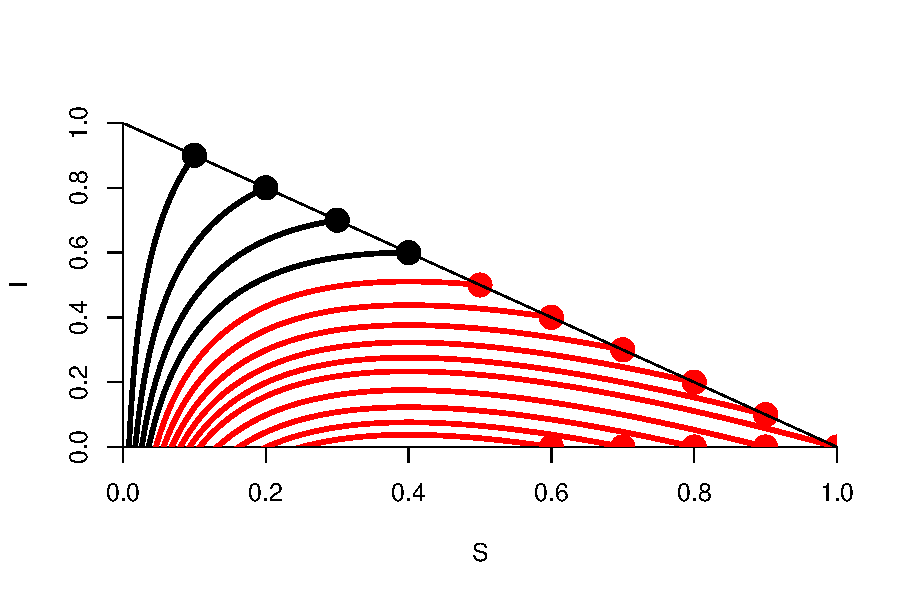
\includegraphics[width=0.9\textwidth]{FIGS/L04-KMK_SI_plane-1.pdf}
\end{center}
\end{frame}



\begin{frame}{}
  Let us study
  $$
  I(S)=S_0+I_0-S+\frac\gamma\beta \ln \frac S{S_0} 
  $$
  We have
  $$
  \frac{d}{dS}I(S) = \frac{\gamma}{\beta S}-1
  $$
  So, in the previous curves, the max of $I(S)$ happens when $S=\gamma/\beta$ ($S=0.4$ in the example)
  \vfill
  At that point,
  $$
  I(S) = I_0+\left(
    1-\frac{1}{\R_0} - \frac{\ln(\R_0)}{\R_0}
  \right)S_0
  $$
\end{frame}


\begin{frame}{}
  \begin{theorem}[Epidemic or no epidemic?]
    Let $(S(t),I(t))$ be a solution to \eqref{sys:KMK_2d} and $\R_0$ defined by
    \begin{equation}\label{eq:R0_KMK}
    \R_0=\frac{\beta}{\gamma}S_0
    \end{equation}
    \vfill
    \begin{itemize}
      \item If $\R_0\leq 1$, then $I(t)\searrow 0$ when $t\to\infty$ 
      \item If $\R_0>1$, then $I(t)$ first reaches a maximum 
      \begin{equation}\label{eq:max_I}
        I_0+\left(
      1-\frac{1}{\R_0} - \frac{\ln(\R_0)}{\R_0}
      \right)S_0
      \end{equation}
      then goes to 0 as $t\to\infty$  
    \end{itemize}    
  \end{theorem}
\end{frame}

\begin{knitrout}
\definecolor{shadecolor}{rgb}{0.969, 0.969, 0.969}\color{fgcolor}\begin{kframe}
\begin{alltt}
\hldef{rhs_SIR_KMK} \hlkwb{<-} \hlkwa{function}\hldef{(}\hlkwc{t}\hldef{,} \hlkwc{x}\hldef{,} \hlkwc{p}\hldef{) \{}
  \hlkwd{with}\hldef{(}\hlkwd{as.list}\hldef{(}\hlkwd{c}\hldef{(x, p)), \{}
    \hldef{dS} \hlkwb{=} \hlopt{-} \hldef{beta} \hlopt{*} \hldef{S} \hlopt{*} \hldef{I}
    \hldef{dI} \hlkwb{=} \hldef{beta} \hlopt{*} \hldef{S} \hlopt{*} \hldef{I} \hlopt{-} \hldef{gamma} \hlopt{*} \hldef{I}
    \hldef{dR} \hlkwb{=} \hldef{gamma} \hlopt{*} \hldef{I}
    \hlkwd{return}\hldef{(}\hlkwd{list}\hldef{(}\hlkwd{c}\hldef{(dS, dI, dR)))}
  \hldef{\})}
\hldef{\}}
\hlcom{# Initial condition for S (to compute R_0)}
\hldef{S0} \hlkwb{=} \hlnum{1000}
\hldef{gamma} \hlkwb{=} \hlnum{1}\hlopt{/}\hlnum{14}
\hlcom{# Set beta so that R_0 = 1.5}
\hldef{beta} \hlkwb{=} \hlnum{1.5} \hlopt{*} \hldef{gamma} \hlopt{/} \hldef{S0}
\hldef{params} \hlkwb{=} \hlkwd{list}\hldef{(}\hlkwc{gamma} \hldef{= gamma,} \hlkwc{beta} \hldef{= beta)}
\hldef{IC} \hlkwb{=} \hlkwd{c}\hldef{(}\hlkwc{S} \hldef{= S0,} \hlkwc{I} \hldef{=} \hlnum{1}\hldef{,} \hlkwc{R} \hldef{=} \hlnum{0}\hldef{)}
\hldef{times} \hlkwb{=} \hlkwd{seq}\hldef{(}\hlnum{0}\hldef{,} \hlnum{365}\hldef{,} \hlnum{1}\hldef{)}
\hldef{sol_KMK} \hlkwb{<-} \hlkwd{ode}\hldef{(IC, times, rhs_SIR_KMK, params)}
\end{alltt}
\end{kframe}
\end{knitrout}



\begin{frame}[fragile]{}
\begin{knitrout}
\definecolor{shadecolor}{rgb}{0.969, 0.969, 0.969}\color{fgcolor}\begin{kframe}
\begin{alltt}
\hlkwd{plot}\hldef{(sol_KMK[,} \hlsng{"time"}\hldef{], sol_KMK[,} \hlsng{"I"}\hldef{],}
     \hlkwc{type} \hldef{=} \hlsng{"l"}\hldef{,} \hlkwc{lwd} \hldef{=} \hlnum{2}\hldef{,}
     \hlkwc{main} \hldef{=} \hlkwd{TeX}\hldef{(}\hlsng{"Kermack-McKendrick SIR, $R_0=1.5$"}\hldef{),}
     \hlkwc{xlab} \hldef{=} \hlsng{"Time (days)"}\hldef{,} \hlkwc{ylab} \hldef{=} \hlsng{"Prevalence"}\hldef{)}
\end{alltt}
\end{kframe}
\end{knitrout}
\begin{center}
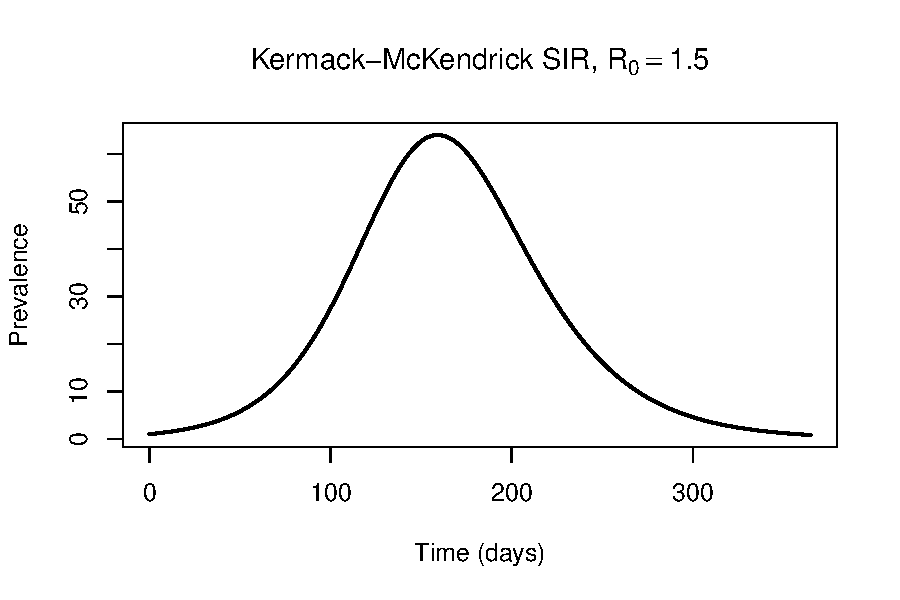
\includegraphics[width=0.8\textwidth]{FIGS/L04-KMK_R0eq1dot5-1.pdf}
\end{center}
\end{frame}


\begin{frame}{The basic reproduction number $\R_0$}
\bbullet Indicator often used in epidemiology. Verbally
\begin{quote}
  average number of secondary cases of infection produced when a single infectious individual is introduced in a wholly susceptible population
\end{quote}
\vfill
\bbullet If $\R_0<1$, then each infectious individual infects on average less than 1 person and the epidemic is quite likely to go extinct 
\vfill
\bbullet If $R_0>1$, then each infectious individual infects on average more than 1 person and an epidemic is quite likely to occur
\end{frame}

\begin{frame}{A few sample values of $\R_0$}
  $\R_0$ can be estimated from data (from the Anderson \& May book)
  \vfill
  \begin{center}
  \begin{tabular}{llcc}
  \hline 
  Infection & Location & Period & $\R_0$ \\
  \hline
  Measles & Cirencester, England & 1947-50 & 13-14 \\
  & England and Wales & 1950-68 & 16-18 \\
  & Kansas, USA & 1918-21 & 5-6 \\
  & Ontario, Canada & 1912-3 & 11-12 \\
  & Willesden, England & 1912-3 & 11-12 \\
  & Ghana & 1960-8 & 14-15 \\
  & East Nigeria & 1960-8 & 16-17 \\
  \end{tabular}
  \end{center}
\end{frame}
    

%%%%%%%%%%%%%%%%%%%%%%%%
%%%%%%%%%%%%%%%%%%%%%%%%
\subsection{The final size of a KMK epidemic}
\newSubSectionSlide{FIGS-slides-admin/Gemini_Generated_Image_vqpscpvqpscpvqps.jpeg}

\begin{frame}{Final size of an epidemic}
  For a nonnegative valued integrable function $w(t)$, denote
  $$
  w_0=w(0),\qquad  w_\infty = \lim_{t\to\infty}w(t),\qquad\hat w = \int_0^\infty w(t)\ dt
  $$
  \vfill
  In the subsystem
  \begin{align}
  S' &= -\beta SI \tag{\ref{sys:KMK_2d_dS}} \\
  I' &= \beta SI-\gamma I \tag{\ref{sys:KMK_2d_dI}} 
  \end{align}
  compute the sum of \eqref{sys:KMK_2d_dS} and \eqref{sys:KMK_2d_dI}, making sure to show time dependence $$
  \frac{d}{dt}(S(t)+I(t))=-\gamma I(t)
  $$
\end{frame}


\begin{frame}{}
  Integrate from 0 to $\infty$:
  $$
  \int_0^\infty\frac{d}{dt}(S(t)+I(t))\ dt=-\int_0^\infty\gamma I(t)dt 
  $$
  The left hand side gives
  $$
  \int_0^\infty\frac{d}{dt}(S(t)+I(t))\ dt
  = S_\infty+I_\infty-S_0-I_0 = S_\infty-S_0-I_0
  $$
  since $I_\infty=0$
  \vfill
  The right hand side takes the form
  $$
  -\int_0^\infty\gamma I(t)dt = -\gamma\int_0^\infty I(t)dt = -\gamma \hat I
  $$
  We thus have
  \begin{equation}
  \label{eq:KMK_final_size_step1}
  S_\infty-S_0-I_0 = -\gamma\hat I
  \end{equation}
\end{frame}



\begin{frame}{}
  Now consider \eqref{sys:KMK_2d_dS}:
  $$
  S' = -\beta SI
  $$
  Divide both sides by $S$:
  $$
  \frac{S'(t)}{S(t)} = -\beta I(t)
  $$
  Integrate from 0 to $\infty$:
  \begin{equation}
  \label{eq:KMK_final_size_step2}
  \ln S_\infty-\ln S_0 = -\beta \hat I
  \end{equation}
  Express \eqref{eq:KMK_final_size_step1} and \eqref{eq:KMK_final_size_step2} in terms of $-\hat I$ and equate
  $$
  \frac{\ln S_\infty-\ln S_0}{\beta}
  =
  \frac{S_\infty-S_0-I_0}{\gamma}
  $$
  Thus we have
  \begin{equation}
  \label{eq:final_size}
  (\ln S_0-\ln S_\infty)S_0 = (S_0-S_\infty)\R_0+I_0\R_0
  \end{equation}
\end{frame}



\begin{frame}{}
\begin{theorem}[Final size relation]
  Let $(S(t),I(t))$ be a solution to \eqref{sys:KMK_2d} and $\R_0$ defined by \eqref{eq:R0_KMK}
  \vskip0.5cm
  The number $S(t)$ of susceptible individuals is a nonincreasing function and its limit $S_\infty$ is the only solution in $(0,S_0)$ of the transcendental equation
  \begin{equation}\tag{\ref{eq:final_size}}
  (\ln S_0-\ln S_\infty)S_0 = (S_0-S_\infty)\R_0+I_0\R_0
  \end{equation}
\end{theorem}
\end{frame}



\begin{frame}{The (transcendantal) final size equation}
  Rewrite the final size equation
  \begin{equation}
    \tag{\ref{eq:final_size}}
  (\ln S_0-\ln S_\infty)S_0 = (S_0-S_\infty)\R_0+I_0\R_0
  \end{equation}
  as
  \begin{equation}
  \label{eq:final_size_2}
  T(S_\infty) =(\ln S_0-\ln S_\infty)S_0
  - (S_0-S_\infty)\R_0 -I_0\R_0
\end{equation}
\vfill
Thus, we seek the zeros of the function $T(S_\infty)$
\end{frame}



\begin{frame}{}
  We seek $S_\infty$ in $(0,S_0]$ s.t. $T(S_\infty)=0$, with
  \begin{equation}\tag{\ref{eq:final_size_2}}
    T(S_\infty) =(\ln S_0-\ln S_\infty)S_0
    - (S_0-S_\infty)\R_0 -I_0\R_0      
  \end{equation}
  \vfill
  Note to begin that 
  $$
  \lim_{S_\infty\to 0}T(S_\infty)=\lim_{S_\infty\to 0}-S_0\ln(S_\infty)=\infty
  $$
  \vfill
  Differentiating $T$ with respect to $S_\infty$, we get 
  $$
  T'(S_\infty)=\R_0-S_0/S_\infty
  $$ 
  \vfill
  When $S_\infty\to 0$, $\R_0-S_0/S_\infty<0$, so $T$ decreases to $S_\infty=S_0/\R_0$
  \vfill
  So if $\R_0\leq 1$, the function $T$ is decreasing on $(0,S_0)$, while it has a minimum if $\R_0>1$
\end{frame}



\begin{frame}{Case $\R_0\leq 1$}
  \begin{equation}\tag{\ref{eq:final_size_2}}
    T(S_\infty) =(\ln S_0-\ln S_\infty)S_0
    - (S_0-S_\infty)\R_0 -I_0\R_0      
  \end{equation}
  \vfill
  \bbullet We have seen that $T$ decreases on $(0,S_0]$
  \vfill
  \bbullet Also, $T(S_0)=-I_0\R_0<0$ ($I_0=0$ is trivial and not considered)
  \vfill
  \bbullet $T$ is continuous
  \vfill
  $\implies$ there exists a unique $S_\infty\in (0,S_0]$ s.t. $T(S_\infty)=0$
\end{frame}


\begin{frame}{Case $\R_0> 1$}
  \begin{equation}\tag{\ref{eq:final_size_2}}
    T(S_\infty) =(\ln S_0-\ln S_\infty)S_0
    - (S_0-S_\infty)\R_0 -I_0\R_0      
  \end{equation}
  \vfill
  \bbullet We have seen that $T$ decreases on $(0,S_0/\R_0]$
  \vfill
  \bbullet For $S_\infty\in[S_0/\R_0]$, $T'>0$
  \vfill
  \bbullet As before, $T(S_\infty)=-I_0\R_0$
  \vfill
  \bbullet $T$ is continuous
  \vfill
  $\implies$ there exists a unique $S_\infty\in (0,S_0]$ s.t. $T(S_\infty)=0$. More precisely, in this case, $S_\infty\in(0,S_0/\R_0)$
\end{frame}



\begin{frame}[fragile]{}
We solve numerically. We need a function
\begin{knitrout}
\definecolor{shadecolor}{rgb}{0.969, 0.969, 0.969}\color{fgcolor}\begin{kframe}
\begin{alltt}
\hldef{final_size_eq} \hlkwb{=} \hlkwa{function}\hldef{(}\hlkwc{S_inf}\hldef{,} \hlkwc{S0} \hldef{=} \hlnum{999}\hldef{,} \hlkwc{I0} \hldef{=} \hlnum{1}\hldef{,} \hlkwc{R_0} \hldef{=} \hlnum{2.5}\hldef{) \{}
  \hldef{OUT} \hlkwb{=} \hldef{S0}\hlopt{*}\hldef{(}\hlkwd{log}\hldef{(S0)}\hlopt{-}\hlkwd{log}\hldef{(S_inf))} \hlopt{-} \hldef{(S0}\hlopt{+}\hldef{I0}\hlopt{-}\hldef{S_inf)}\hlopt{*}\hldef{R_0}
  \hlkwd{return}\hldef{(OUT)}
\hldef{\}}
\end{alltt}
\end{kframe}
\end{knitrout}
and solve easily using \code{uniroot}:
\begin{knitrout}
\definecolor{shadecolor}{rgb}{0.969, 0.969, 0.969}\color{fgcolor}\begin{kframe}
\begin{alltt}
\hlkwd{uniroot}\hldef{(}\hlkwc{f} \hldef{= final_size_eq,} \hlkwc{interval} \hldef{=} \hlkwd{c}\hldef{(}\hlnum{0.05}\hldef{,} \hlnum{999}\hldef{))}
\end{alltt}
\begin{verbatim}
## $root
## [1] 106.8819
## 
## $f.root
## [1] -2.649285e-07
## 
## $iter
## [1] 10
## 
## $init.it
## [1] NA
## 
## $estim.prec
## [1] 6.103516e-05
\end{verbatim}
\end{kframe}
\end{knitrout}
\end{frame}


\begin{frame}[fragile]{A function to use this..}
\begin{knitrout}
\definecolor{shadecolor}{rgb}{0.969, 0.969, 0.969}\color{fgcolor}\begin{kframe}
\begin{alltt}
\hldef{final_size} \hlkwb{=} \hlkwa{function}\hldef{(}\hlkwc{L}\hldef{) \{}
  \hlkwd{with}\hldef{(}\hlkwd{as.list}\hldef{(L), \{}
  \hldef{S_inf} \hlkwb{=} \hlkwd{uniroot}\hldef{(}\hlkwc{f} \hldef{=} \hlkwa{function}\hldef{(}\hlkwc{x}\hldef{)}
    \hlkwd{final_size_eq}\hldef{(}\hlkwc{S_inf} \hldef{= x,}
                  \hlkwc{S0} \hldef{= S0,} \hlkwc{I0} \hldef{= I0,}
                  \hlkwc{R_0} \hldef{= R_0),}
    \hlkwc{interval} \hldef{=} \hlkwd{c}\hldef{(}\hlnum{0.05}\hldef{, S0))}
  \hlkwd{return}\hldef{(S_inf}\hlopt{$}\hldef{root)}
  \hldef{\})}
\hldef{\}}
\end{alltt}
\end{kframe}
\end{knitrout}
\end{frame}

\begin{frame}[fragile]{A figure with all the information}
\begin{knitrout}
\definecolor{shadecolor}{rgb}{0.969, 0.969, 0.969}\color{fgcolor}\begin{kframe}
\begin{alltt}
\hldef{N0} \hlkwb{=} \hlnum{1000}
\hldef{I0} \hlkwb{=} \hlnum{1}
\hldef{S0} \hlkwb{=} \hldef{N0}\hlopt{-}\hldef{I0}
\hldef{R_0} \hlkwb{=} \hlnum{0.8}
\hldef{S} \hlkwb{=} \hlkwd{seq}\hldef{(}\hlnum{0.1}\hldef{, S0,} \hlkwc{by} \hldef{=} \hlnum{0.1}\hldef{)}
\hldef{fs} \hlkwb{=} \hlkwd{final_size_eq}\hldef{(S,} \hlkwc{S0} \hldef{= S0,} \hlkwc{I0} \hldef{= I0,} \hlkwc{R_0} \hldef{= R_0)}
\hldef{S_inf} \hlkwb{=} \hlkwd{uniroot}\hldef{(}\hlkwc{f} \hldef{=} \hlkwa{function}\hldef{(}\hlkwc{x}\hldef{)} \hlkwd{final_size_eq}\hldef{(}\hlkwc{S_inf} \hldef{= x,}
                                              \hlkwc{S0} \hldef{= S0,} \hlkwc{I0} \hldef{= I0,}
                                              \hlkwc{R_0} \hldef{= R_0),}
                \hlkwc{interval} \hldef{=} \hlkwd{c}\hldef{(}\hlnum{0.05}\hldef{, S0))}
\hlkwd{plot}\hldef{(S, fs,} \hlkwc{type} \hldef{=} \hlsng{"l"}\hldef{,} \hlkwc{ylab} \hldef{=} \hlsng{"Value of equation (10)"}\hldef{)}
\hlkwd{abline}\hldef{(}\hlkwc{h} \hldef{=} \hlnum{0}\hldef{)}
\hlkwd{points}\hldef{(}\hlkwc{x} \hldef{= S_inf}\hlopt{$}\hldef{root,} \hlkwc{y} \hldef{=} \hlnum{0}\hldef{,} \hlkwc{pch} \hldef{=} \hlnum{19}\hldef{)}
\hlkwd{text}\hldef{(}\hlkwc{x} \hldef{= S_inf}\hlopt{$}\hldef{root,} \hlkwc{y} \hldef{=} \hlnum{0}\hldef{,} \hlkwc{labels} \hldef{=} \hlsng{"S_inf"}\hldef{,} \hlkwc{adj} \hldef{=} \hlkwd{c}\hldef{(}\hlopt{-}\hlnum{0.25}\hldef{,}\hlopt{-}\hlnum{1}\hldef{))}
\end{alltt}
\end{kframe}
\end{knitrout}
\end{frame}



\begin{frame}{$\R_0=0.8$}
\begin{center}
  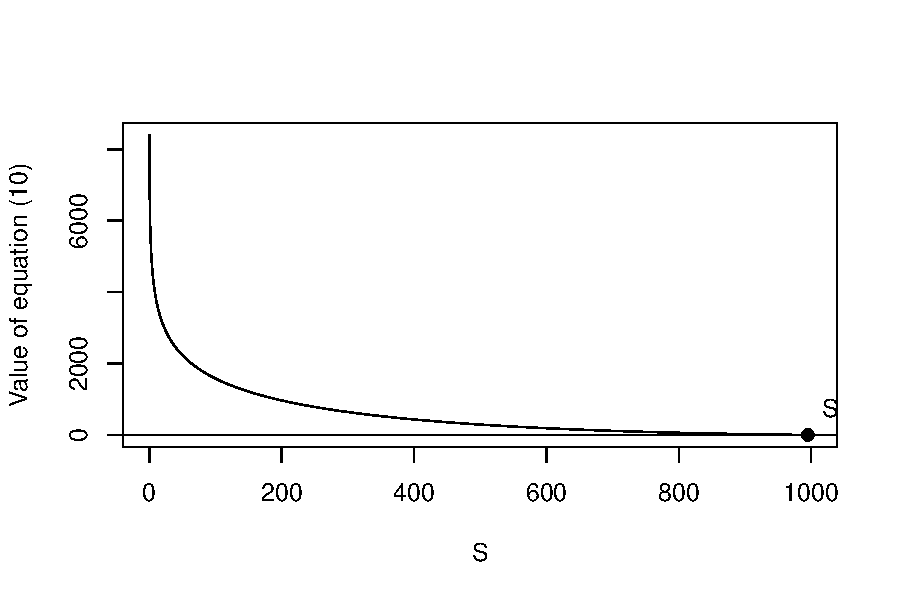
\includegraphics[width=\textwidth]{FIGS/L04-KMK_final_size_0p8-1.pdf}
\end{center}
\end{frame}





\begin{frame}{$\R_0=2.4$}
  \begin{center}
    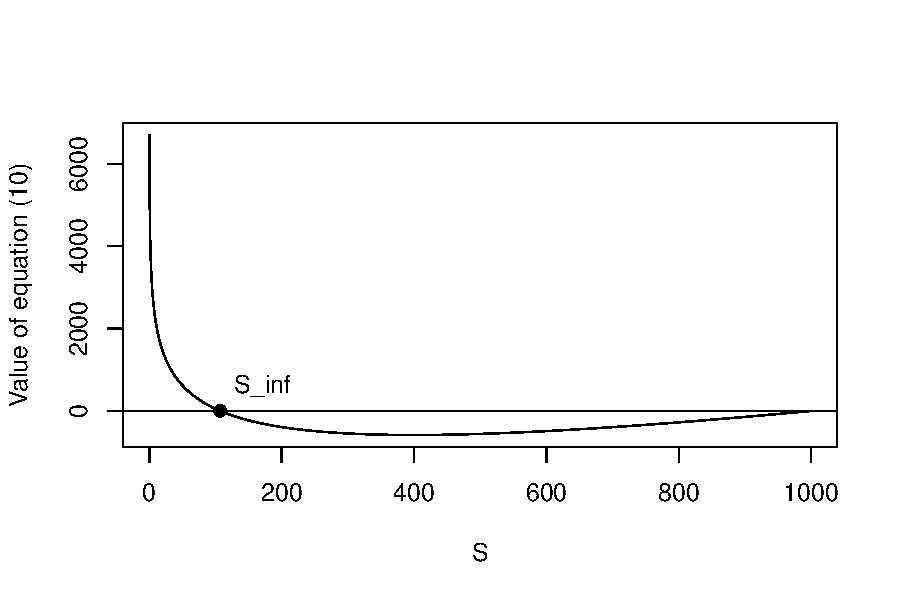
\includegraphics[width=\textwidth]{FIGS/L04-KMK_final_size_2p5-1.pdf}
  \end{center}
\end{frame}

\begin{frame}[fragile]{A little nicer}
\begin{knitrout}
\definecolor{shadecolor}{rgb}{0.969, 0.969, 0.969}\color{fgcolor}\begin{kframe}
\begin{alltt}
\hldef{values} \hlkwb{=} \hlkwd{expand.grid}\hldef{(}
  \hlkwc{R_0} \hldef{=} \hlkwd{seq}\hldef{(}\hlnum{0.01}\hldef{,} \hlnum{3}\hldef{,} \hlkwc{by} \hldef{=} \hlnum{0.01}\hldef{),}
  \hlkwc{I0} \hldef{=} \hlkwd{seq}\hldef{(}\hlnum{1}\hldef{,} \hlnum{100}\hldef{,} \hlnum{1}\hldef{)}
\hldef{)}
\hldef{values}\hlopt{$}\hldef{S0} \hlkwb{=} \hldef{N0}\hlopt{-}\hldef{values}\hlopt{$}\hldef{I0}
\hldef{L} \hlkwb{=} \hlkwd{split}\hldef{(values,} \hlnum{1}\hlopt{:}\hlkwd{nrow}\hldef{(values))}
\hldef{values}\hlopt{$}\hldef{S_inf} \hlkwb{=} \hlkwd{sapply}\hldef{(}\hlkwc{X} \hldef{= L,} \hlkwc{FUN} \hldef{= final_size)}
\hldef{values}\hlopt{$}\hldef{final_size} \hlkwb{=} \hldef{values}\hlopt{$}\hldef{S0}\hlopt{-}\hldef{values}\hlopt{$}\hldef{S_inf}\hlopt{+}\hldef{values}\hlopt{$}\hldef{I0}
\hldef{values}\hlopt{$}\hldef{attack_rate} \hlkwb{=} \hldef{(values}\hlopt{$}\hldef{final_size} \hlopt{/} \hldef{N0)}\hlopt{*}\hlnum{100}

\hldef{p} \hlkwb{=} \hlkwd{levelplot}\hldef{(attack_rate} \hlopt{~} \hldef{R_0}\hlopt{*}\hldef{I0,} \hlkwc{data} \hldef{= values,}
              \hlkwc{xlab} \hldef{=} \hlkwd{TeX}\hldef{(}\hlsng{"$R_0$"}\hldef{),} \hlkwc{ylab} \hldef{=} \hlsng{"I(0)"}\hldef{,}
              \hlkwc{col.regions} \hldef{=} \hlkwd{viridis}\hldef{(}\hlnum{100}\hldef{))}
\hlkwd{print}\hldef{(p)}
\end{alltt}
\end{kframe}
\end{knitrout}
(requires \code{lattice}, \code{viridis} and \code{latex2exp} librairies)
\end{frame}

\begin{frame}{Attack rate (in \%)}
  \begin{center}
    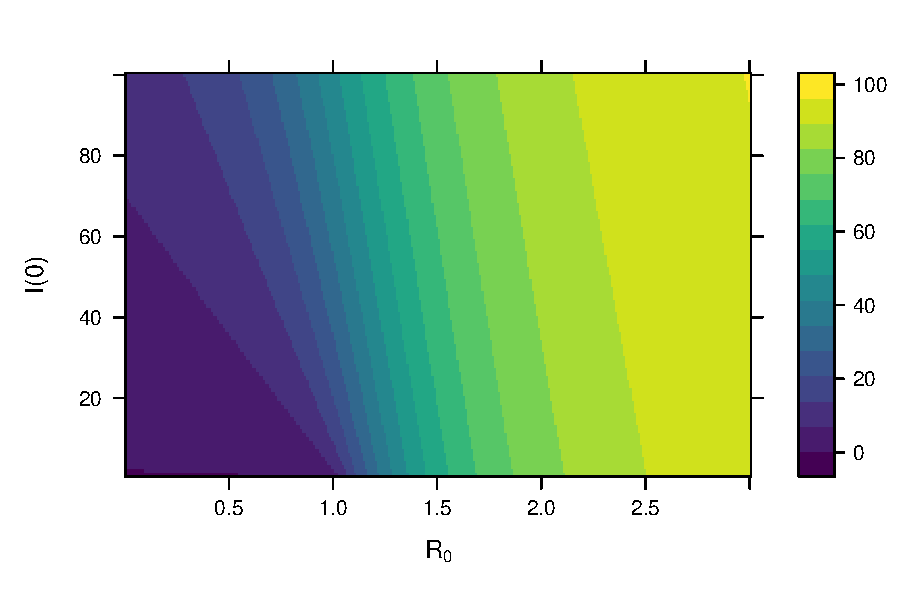
\includegraphics[width=0.9\textwidth]{FIGS/L04-KMK_attack_rate-1.pdf}
  \end{center}
\end{frame}


%%%%%%%%%%%%%%%%%%%%%%%%%%%
%%%%%%%%%%%%%%%%%%%%%%%%%%%
\subsection{Herd immunity in KMK}
\newSubSectionSlide{FIGS-slides-admin/Gemini_Generated_Image_vqpscpvqpscpvqps.jpeg}


\begin{frame}{The simplest vaccination model}
To implement vaccination in KMK, assume that vaccination reduces the number of susceptibles
\vfill
Let total population be $N$ with $S_0$ initially susceptible
\vfill
Vaccinate a fraction $p\in[0,1]$ of susceptible individuals
\vfill
Original IC (for simplicity, $R(0)=0$)
\begin{equation}\label{eq:IC_KMK_novacc}
IC: (S(0),I(0),R(0)) = (S_0,I_0,0)
\end{equation}
Post-vaccination IC 
\begin{equation}\label{eq:IC_KMK_vacc}
IC: (S(0),I(0),R(0)) = ((1-p)S_0,I_0,pS_0)
\end{equation}
\end{frame}


\begin{frame}{Vaccination reproduction number}
  Without vaccination
  \begin{equation}\tag{\ref{eq:R0_KMK}}
    \R_0=\frac{\beta}{\gamma}S_0
  \end{equation}
  \vfill
  With vaccination, denoting $\R_{\text{v}}$ the reproduction number,
  \begin{equation}
    \R_{\text{v}} = \frac{\beta}{\gamma}(1-p)S_0
  \end{equation}
  \vfill
  Since $p\in[0,1]$, $\R_{\text{v}}\leq\R_0$
\end{frame}


\begin{frame}{Herd immunity}
  Therefore
  \begin{itemize}
    \item $\R_{\text{v}}<\R_0$ if $p>0$ 
    \item To control the disease, $\R_{\text{v}}$ must take a value less than 1
  \end{itemize}
  \vfill
To make $\R_{\text{v}}$ less than 1
  \begin{equation}\label{eq:herd_immunity}
    \R_{\text{v}}<1 \iff p> 1-\frac{1}{\R_0}
  \end{equation}
  \vfill
  By vaccinating a fraction $p>1-1/\R_0$ of the susceptible population, we thus are in a situation where an epidemic peak is precluded (or, at the very least, the final size is reduced)
  \vfill
  This is \defword{herd immunity}
\end{frame}


\begin{knitrout}
\definecolor{shadecolor}{rgb}{0.969, 0.969, 0.969}\color{fgcolor}\begin{kframe}
\begin{verbatim}
## [1] "../CODE/L04-KMK-intro.R"
\end{verbatim}
\end{kframe}
\end{knitrout}



\begin{frame}[allowframebreaks]{Bibliography}
\bibliographystyle{plain}
\bibliography{local-bibliography}
\end{frame}

\end{document}
